\documentclass[a4paper,12pt,landscape,twocolumn]{article}

\usepackage{préambule}
\usepackage{clipboard}

\renewcommand{\arraystretch}{1.3}

\begin{document}

\Copy{exemple}{
\begin{exemple}
	Voici les notes d'un devoir de mathématiques:

	\begin{center}
		\begin{tabular}{|l|c|c|c|c|c|c|c|c|c|}
			\hline
			Note     & 2 & 3 & 4 & 5 & 6 & 7 & 8 & 9 & 10
			\\ \hline
			Effectif & 2 & 3 & 1 & 4 & 5 & 3 & 3 & 6 & 2
			\\ \hline
		\end{tabular}
	\end{center}

	À chaque note est associé un bâton : sa hauteur est le nombre d'élèves ayant obtenu cette note.

	\begin{center}
		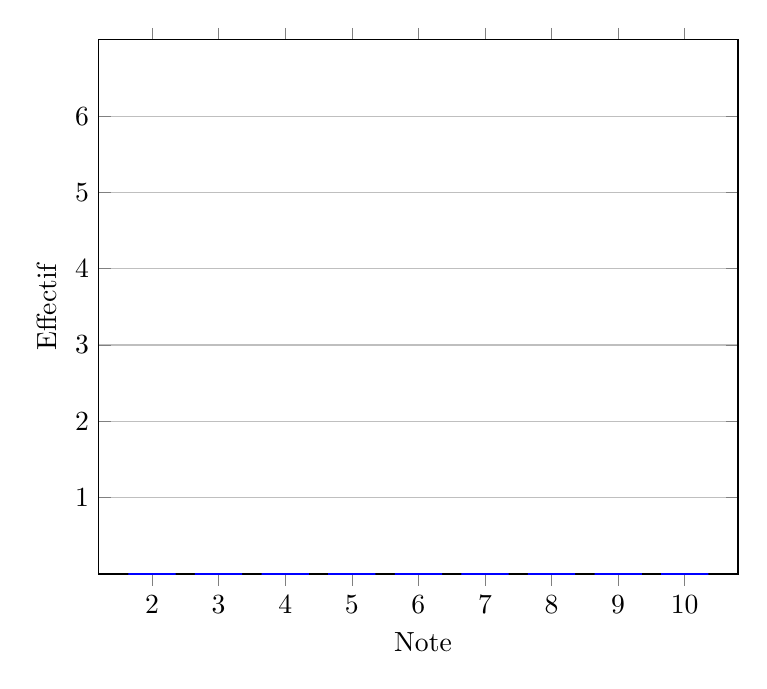
\begin{tikzpicture}
			\begin{axis}[
					width = 0.8\textwidth,
					ybar,
					bar width=0.6cm,
					ymin=0, ymax=7,
					ylabel={Effectif},
					xlabel={\ Note},
					symbolic x coords={2, 3, 4, 5, 6, 7, 8, 9, 10},
					xtick=data,
					ymajorgrids = true,
					scaled y ticks = false,
					ytick={1,2,3,4,5,6},
				]
				\addplot coordinates { (2,0) (3,0) (4,0) (5,0) (6,0) (7,0) (8,0) (9,0) (10,0) };
			\end{axis}
		\end{tikzpicture}
	\end{center}
\end{exemple}
}

\newpage
\Paste{exemple}

\end{document}